\documentclass[12pt,a4paper]{article}
\usepackage{fontspec}
\IfFontExistsTF{Times New Roman}{\setmainfont{Times New Roman}}{\setmainfont{CMU Serif}}
\IfFontExistsTF{Arial}{\setsansfont{Arial}}{\setsansfont{CMU Sans Serif}}
\usepackage[russian]{babel}
\usepackage[margin=18mm]{geometry}
\usepackage{amsmath,amssymb,graphicx,booktabs}
\usepackage{setspace}
\usepackage{titlesec}
\titlespacing*{\section}{0pt}{9pt}{4pt}
\titlespacing*{\subsection}{0pt}{6pt}{3pt}
\setlength{\abovedisplayskip}{5pt}
\setlength{\belowdisplayskip}{5pt}
\usepackage[unicode,hidelinks]{hyperref}
\setstretch{1.05}
\setlength{\parindent}{1cm}
\setlength{\emergencystretch}{2em}
\begin{document}
\begin{center}
{\large\bfseries Лабораторная работа №1. Цветовые модели}\\
Ходько Мария Дмитриевна, группа 3\\
Чётный вариант: CMYK — RGB — HSV
\end{center}
\section{Цель работы}
Изучить цветовые модели RGB, CMYK и HSV, реализовать преобразования между ними и разработать приложение для интерактивного задания цвета с автоматическим пересчётом его компонентов.

\section{Постановка задачи}
Создать приложение, одновременно отображающее цвет в трёх моделях. В каждой модели обеспечить три способа задания цвета: числовые поля, ползунки и палитру. Изменение любой компоненты должно автоматически обновлять две остальные модели и образец цвета.

\section{Цветовые модели}
\textbf{RGB} — сложение красного, зелёного и синего света. Каждый канал изменяется от 0 до 255. Чёрный: $(0,0,0)$, белый: $(255,255,255)$.

\textbf{CMYK} — модель печатных красок: голубой C, пурпурной M, жёлтой Y и чёрной K. Диапазон компонентов: 0–100\%. В работе используется математическая модель без профилей печати.

\textbf{HSV} — тон H (0–360$^\circ$), насыщенность S (0–100\%) и яркость V (0–100\%). При S = 0 цвет серый, при V = 0 — чёрный. Тоны 0$^\circ$ и 360$^\circ$ совпадают.
\section{Формулы преобразования}
\subsection{RGB $\to$ CMYK}
Нормируем каналы: $r=R/255$, $g=G/255$, $b=B/255$. Тогда
\[k=1-\max(r,g,b).\]
При $k=1$ принимаем $c=m=y=0$, исключая деление на ноль. Иначе
\[c=\frac{1-r-k}{1-k},\qquad m=\frac{1-g-k}{1-k},\qquad y=\frac{1-b-k}{1-k}.\]
Отображаемые проценты равны $100c$, $100m$, $100y$, $100k$.
\subsection{CMYK $\to$ RGB}
После перевода процентов в доли единицы:
\[R=255(1-c)(1-k),\quad G=255(1-m)(1-k),\quad B=255(1-y)(1-k).\]
Представление CMYK неоднозначно. Поэтому введённые пользователем компоненты CMYK сохраняются, а при переходе из RGB выбирается представление с $k=1-\max(r,g,b)$.
\subsection{RGB $\to$ HSV}
Обозначим $M=\max(r,g,b)$, $m=\min(r,g,b)$, $\Delta=M-m$.
\[V=100M,\qquad S=\begin{cases}0,&M=0,\\100\Delta/M,&M\ne0.\end{cases}\]
\[H=\begin{cases}0,&\Delta=0,\\60\bigl(((g-b)/\Delta)\bmod6\bigr),&M=r,\ \Delta\ne0,\\60((b-r)/\Delta+2),&M=g,\ \Delta\ne0,\\60((r-g)/\Delta+4),&M=b,\ \Delta\ne0.\end{cases}\]
Отрицательный угол приводится к диапазону $[0,360)$ прибавлением $360^\circ$. Для ахроматического цвета функция возвращает условный тон $0^\circ$; интерфейс сохраняет предыдущий тон, поскольку при $S=0$ он не влияет на цвет.
\subsection{HSV $\to$ RGB}
Пусть $s=S/100$, $v=V/100$, $H\in[0,360)$. Вычислим
\[C=vs,\qquad X=C\left(1-\left|((H/60)\bmod2)-1\right|\right),\qquad t=v-C.\]
\[(r_1,g_1,b_1)=\begin{cases}(C,X,0),&0\le H<60,\\(X,C,0),&60\le H<120,\\(0,C,X),&120\le H<180,\\(0,X,C),&180\le H<240,\\(X,0,C),&240\le H<300,\\(C,0,X),&300\le H<360.\end{cases}\]
\[R=255(r_1+t),\qquad G=255(g_1+t),\qquad B=255(b_1+t).\]
Преобразования CMYK $\leftrightarrow$ HSV выполняются через RGB.

\section{Реализация приложения}
Приложение создано на HTML, CSS и JavaScript. Для запуска нужно открыть \texttt{index.html} в браузере. Формулы находятся в \texttt{color.js}, обработчики интерфейса — в \texttt{app.js}.

В каждой модели доступны числовые поля, ползунки и палитра. При изменении любой компоненты автоматически пересчитываются две другие модели и обновляется образец цвета. Дополнительно доступны HEX-код и готовые цвета. Палитра браузера передаёт выбранный цвет в RGB, после чего вычисляются CMYK и HSV.

Значения вне диапазона ограничиваются допустимыми границами. Некорректный ввод не меняет цвет. Вычисления выполняются без промежуточного округления; числа в полях отображаются с точностью до двух знаков.
\section{Проверка преобразований}
Автоматическая проверка выполняет непосредственно JavaScript-код из color.js в системном движке JavaScriptCore macOS. Проверены шесть контрольных цветов, 10 000 наборов RGB с воспроизводимой генерацией, обратные преобразования RGB $\to$ CMYK $\to$ RGB и RGB $\to$ HSV $\to$ RGB, а также H = 360$^\circ$. Допустимое абсолютное отклонение составляет 10$^{-8}$ на компоненту. Все проверки пройдены.

Контрольные значения (проценты округлены до двух знаков):

\begin{center}\small\begin{tabular}{llll}\toprule
Цвет & RGB & CMYK, \% & HSV, $^\circ$ / \% / \% \\
Чёрный & 0, 0, 0 & 0, 0, 0, 100 & 0, 0, 0 \\
Белый & 255, 255, 255 & 0, 0, 0, 0 & 0, 0, 100 \\
Красный & 255, 0, 0 & 0, 100, 100, 0 & 0, 100, 100 \\
Зелёный & 0, 255, 0 & 100, 0, 100, 0 & 120, 100, 100 \\
Синий & 0, 0, 255 & 100, 100, 0, 0 & 240, 100, 100 \\
Серый & 128, 128, 128 & 0, 0, 0, 49.80 & 0, 0, 50.20 \\
\bottomrule\end{tabular}\end{center}

В таблице для ахроматических цветов указан условный тон 0$^\circ$. В интерфейсе для них может сохраняться предыдущий тон: при S = 0 это не влияет на цвет.

\section{Скриншоты приложения}
На рисунках показаны интерфейс и примеры задания цвета в RGB, CMYK и HSV.
\begin{center}
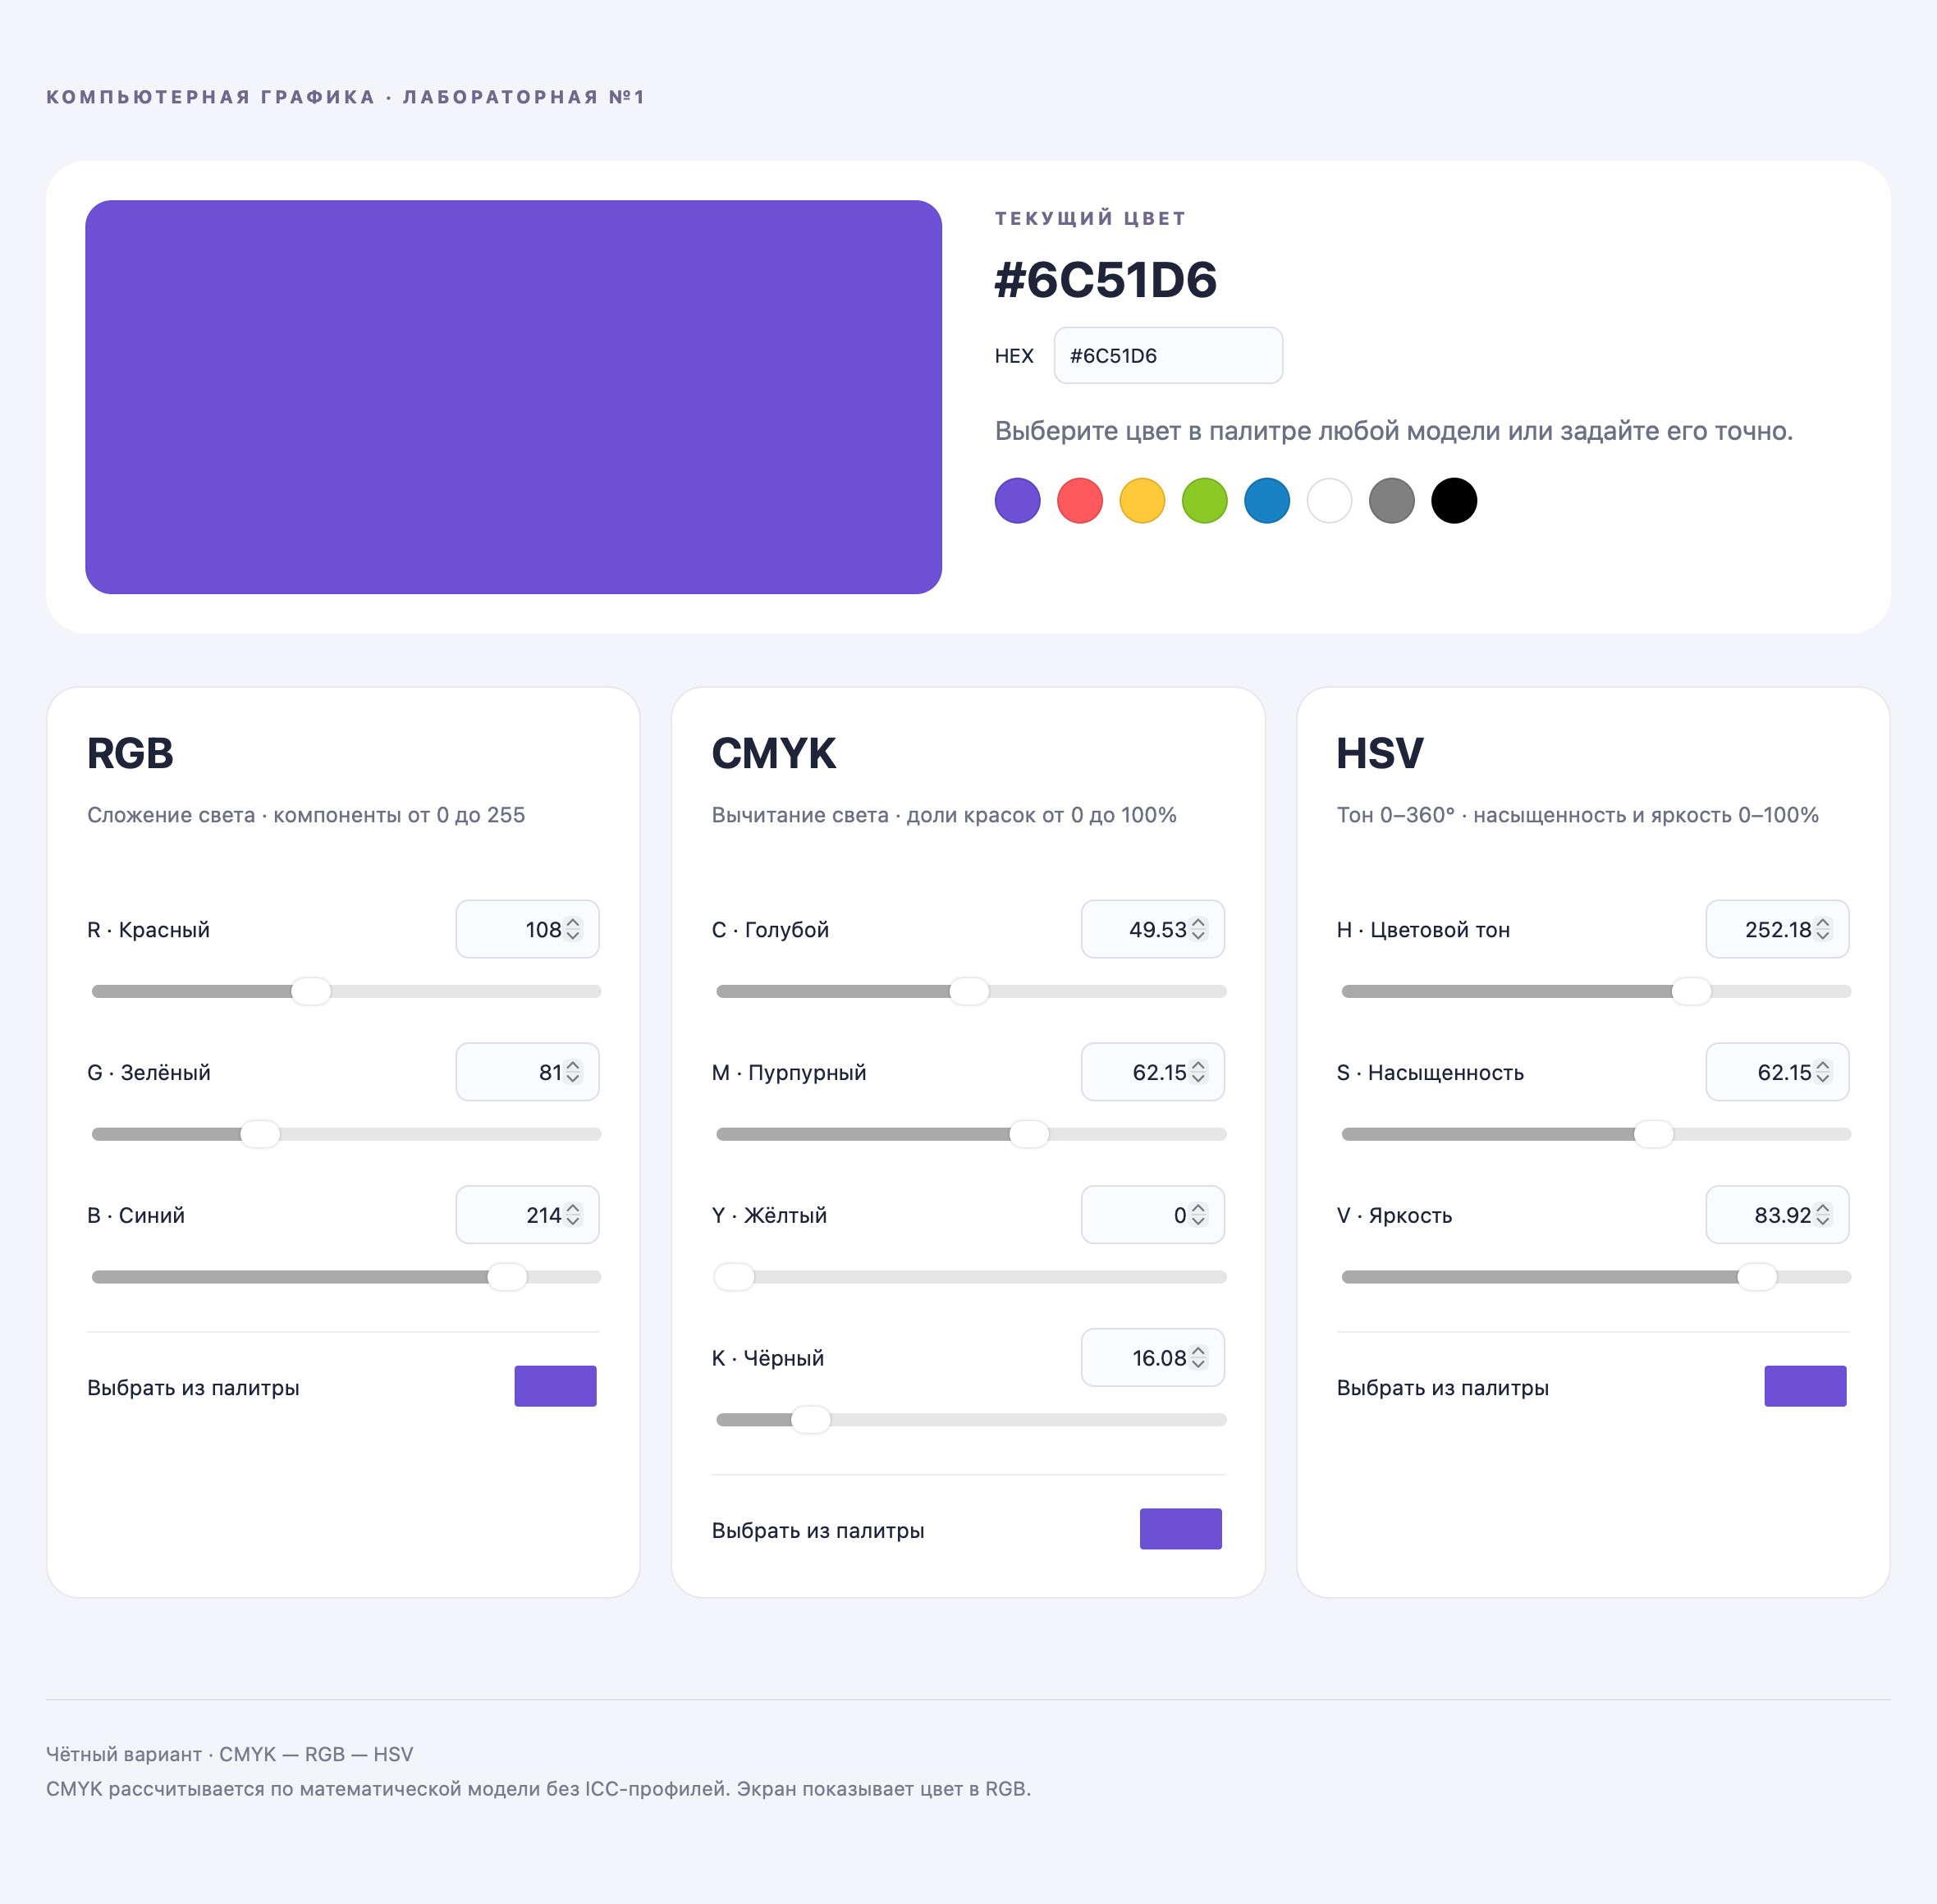
\includegraphics[width=0.66\textwidth]{screenshots/01-overview.png}\\
{\small Рисунок 1 — Общий вид приложения.}
\end{center}
\begin{center}
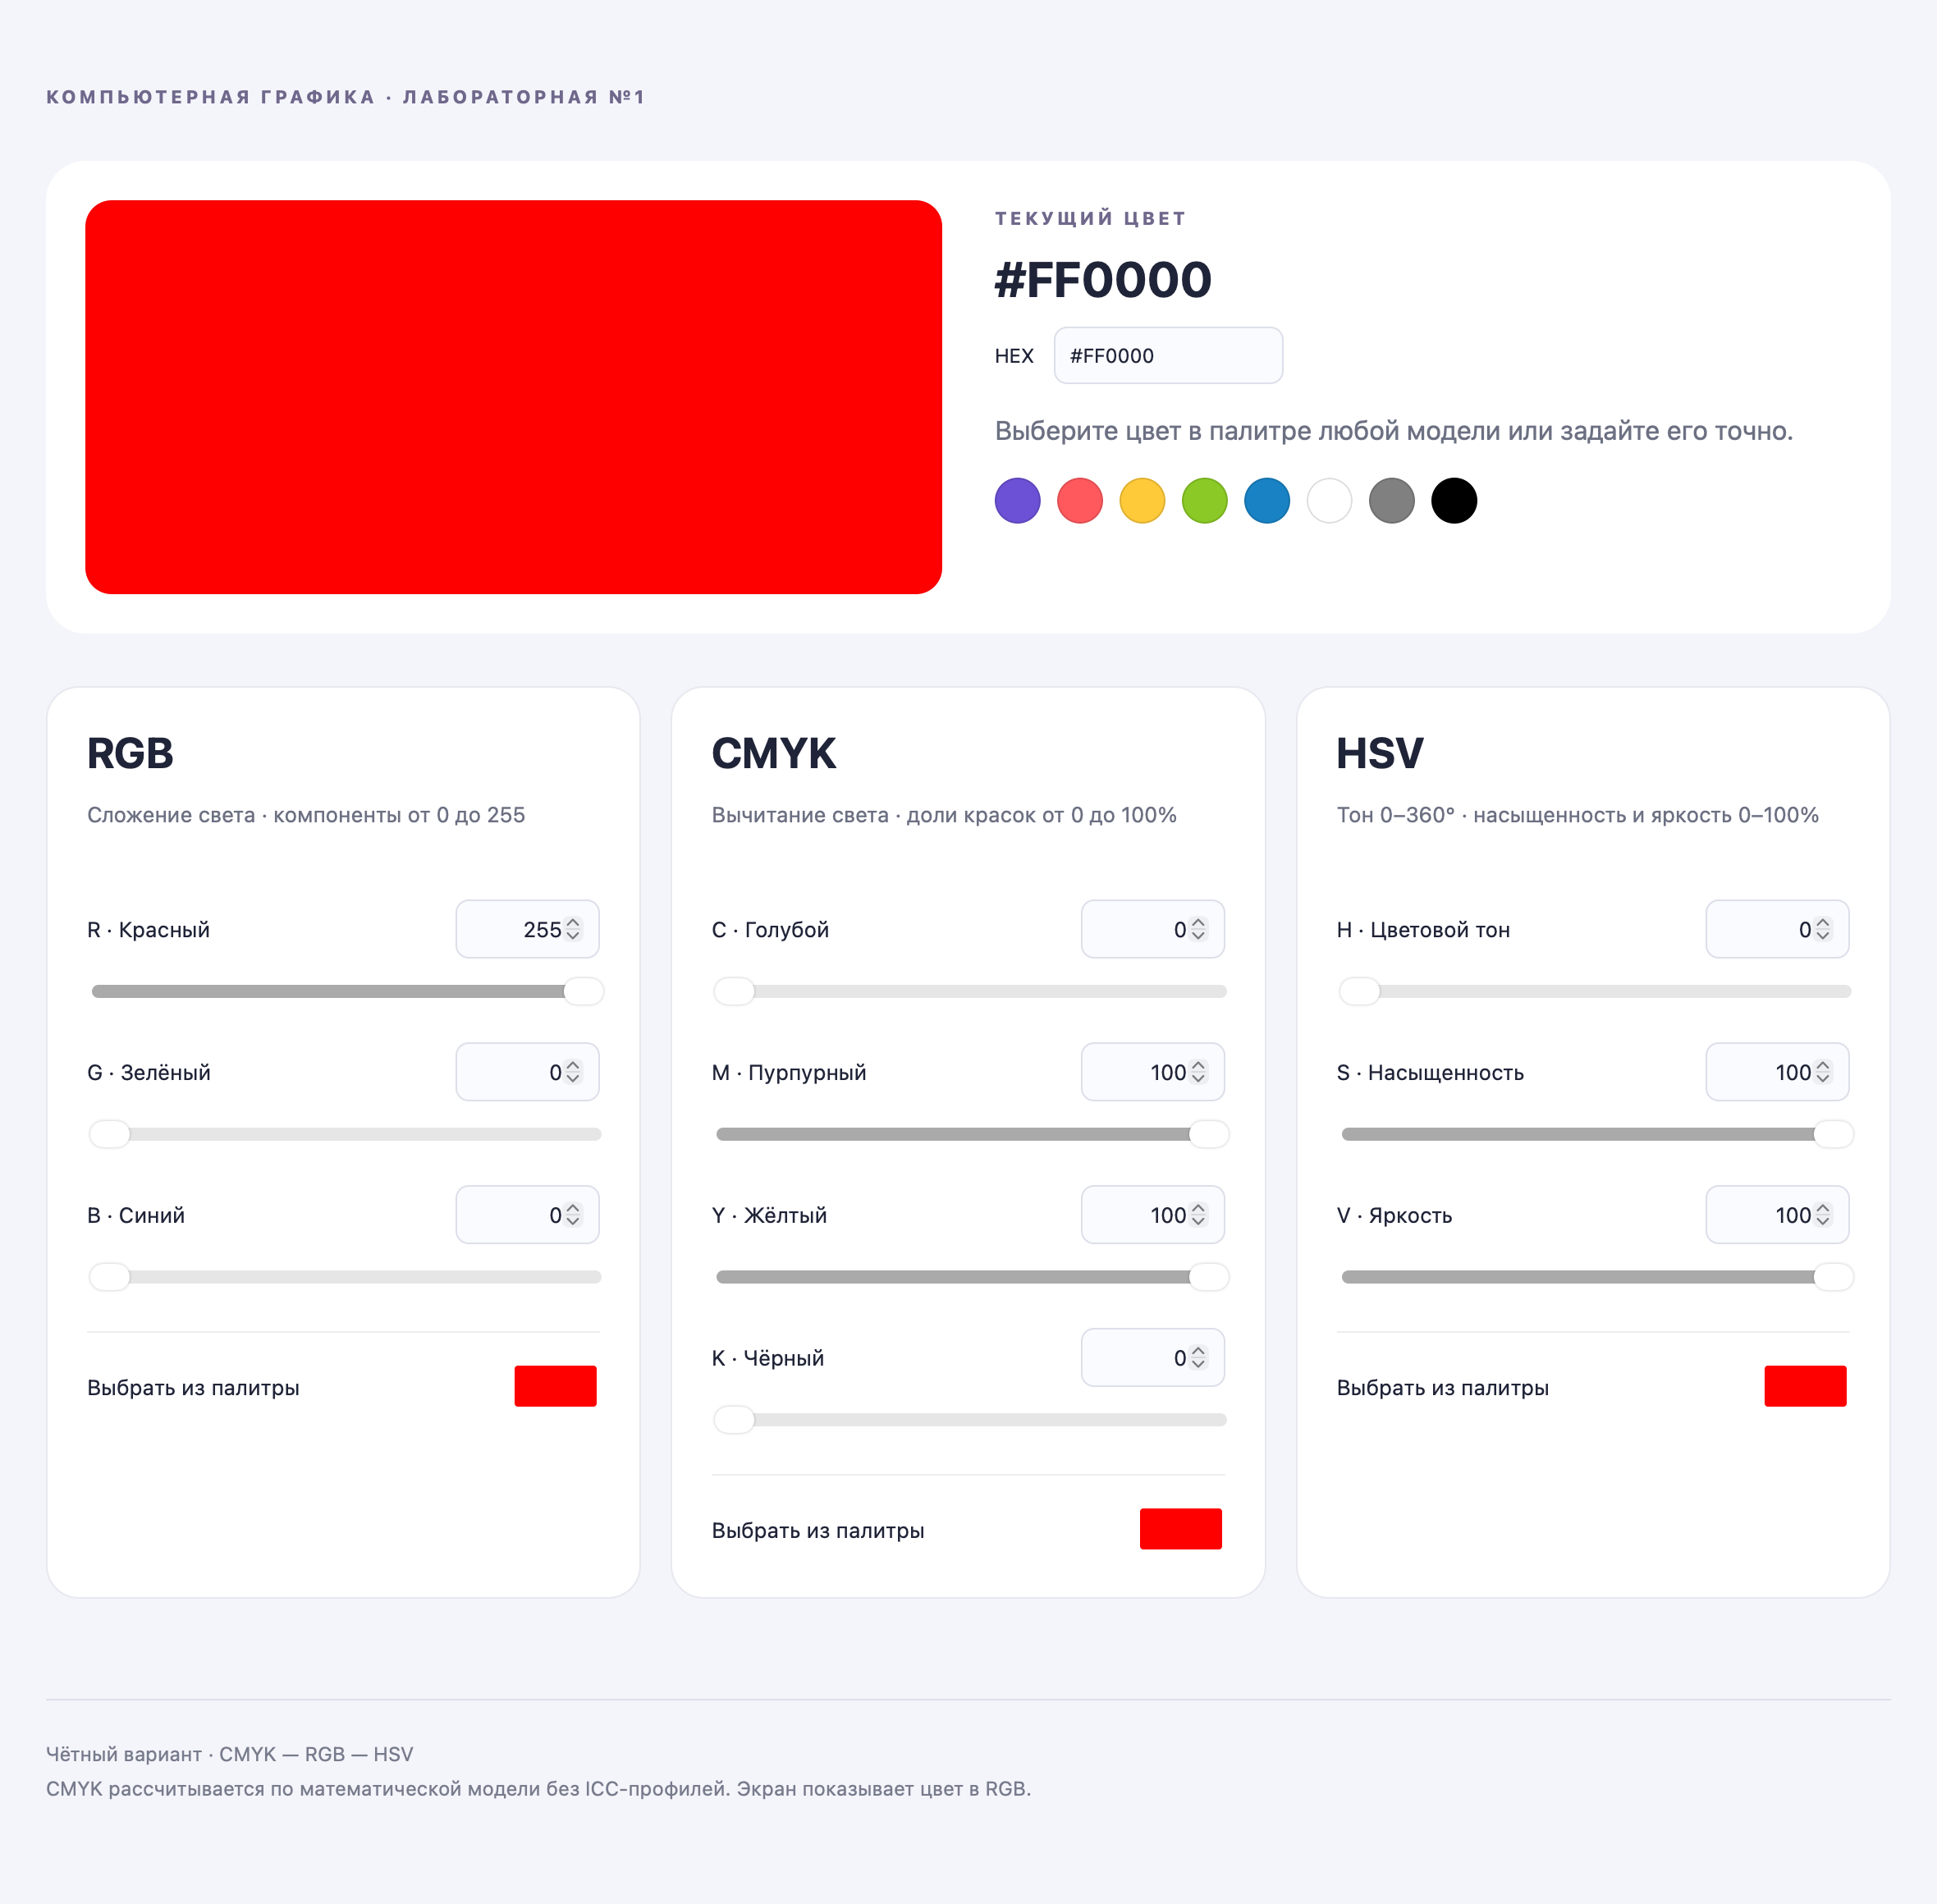
\includegraphics[width=0.66\textwidth]{screenshots/02-rgb-red.png}\\
{\small Рисунок 2 — RGB $(255,0,0)$; CMYK $(0,100,100,0)$; HSV $(0,100,100)$.}
\end{center}
\begin{center}
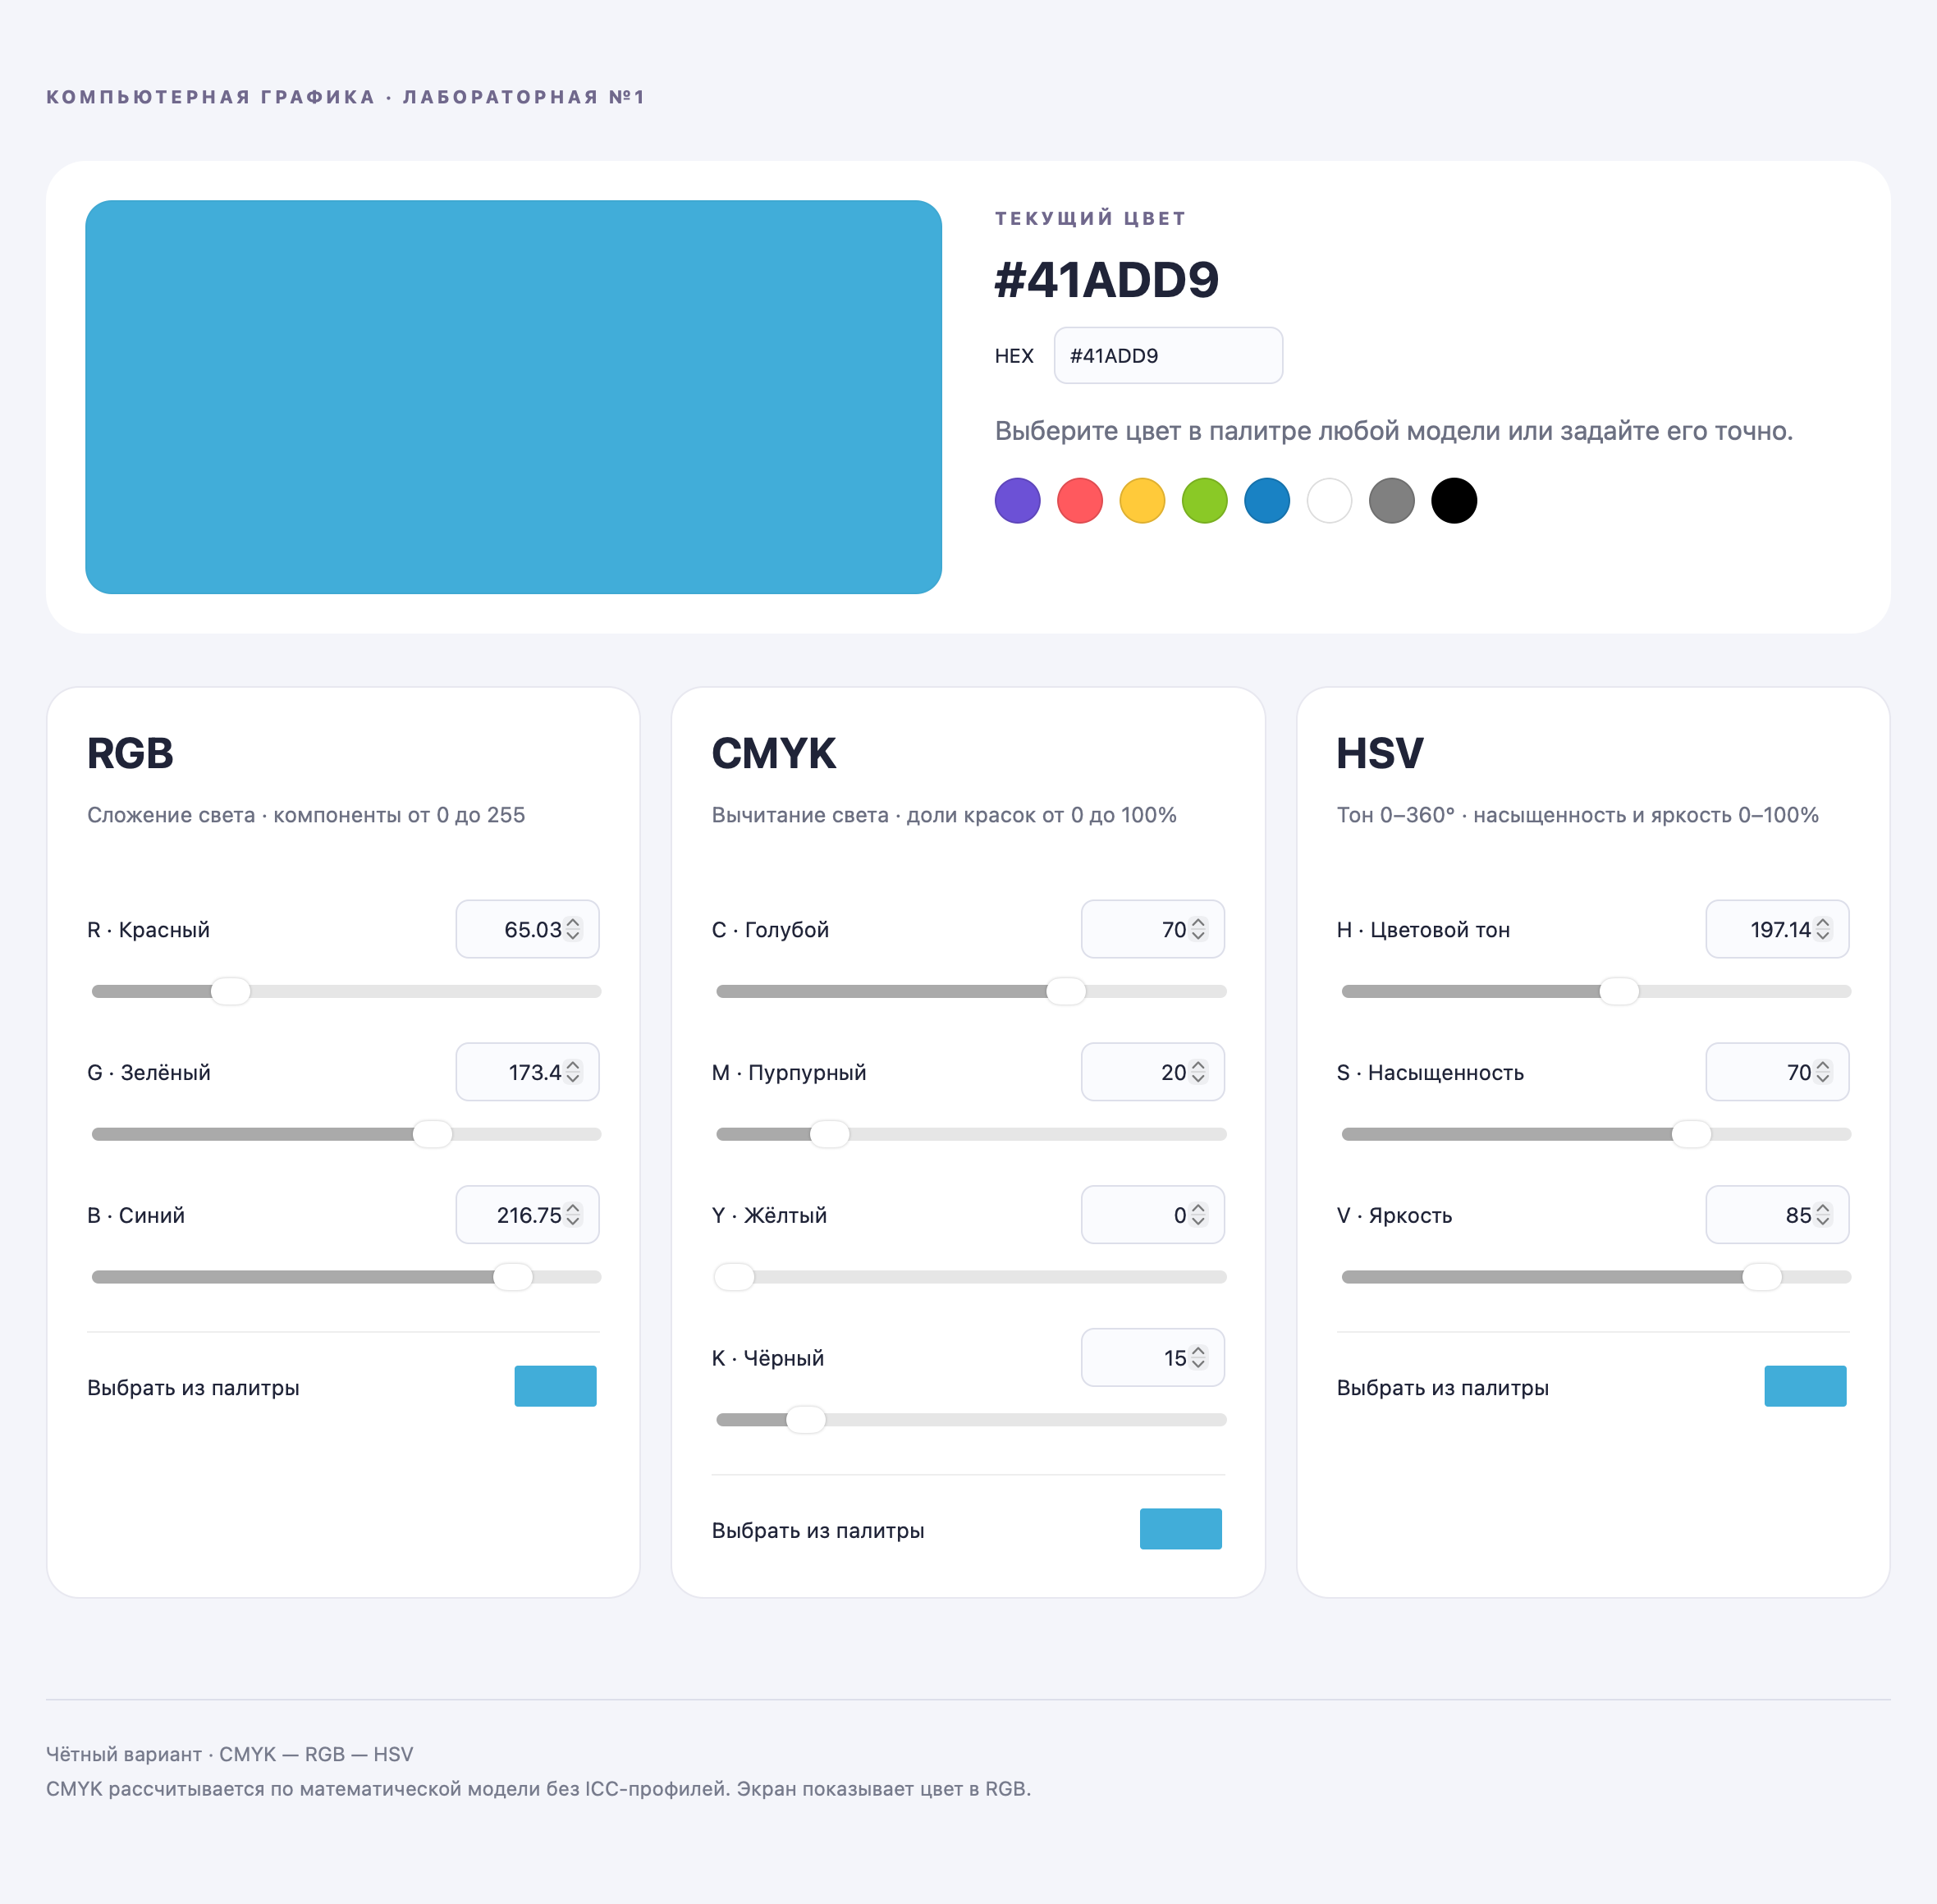
\includegraphics[width=0.66\textwidth]{screenshots/03-cmyk.png}\\
{\small Рисунок 3 — Задание цвета через CMYK $(70,20,0,15)$.}
\end{center}
\begin{center}
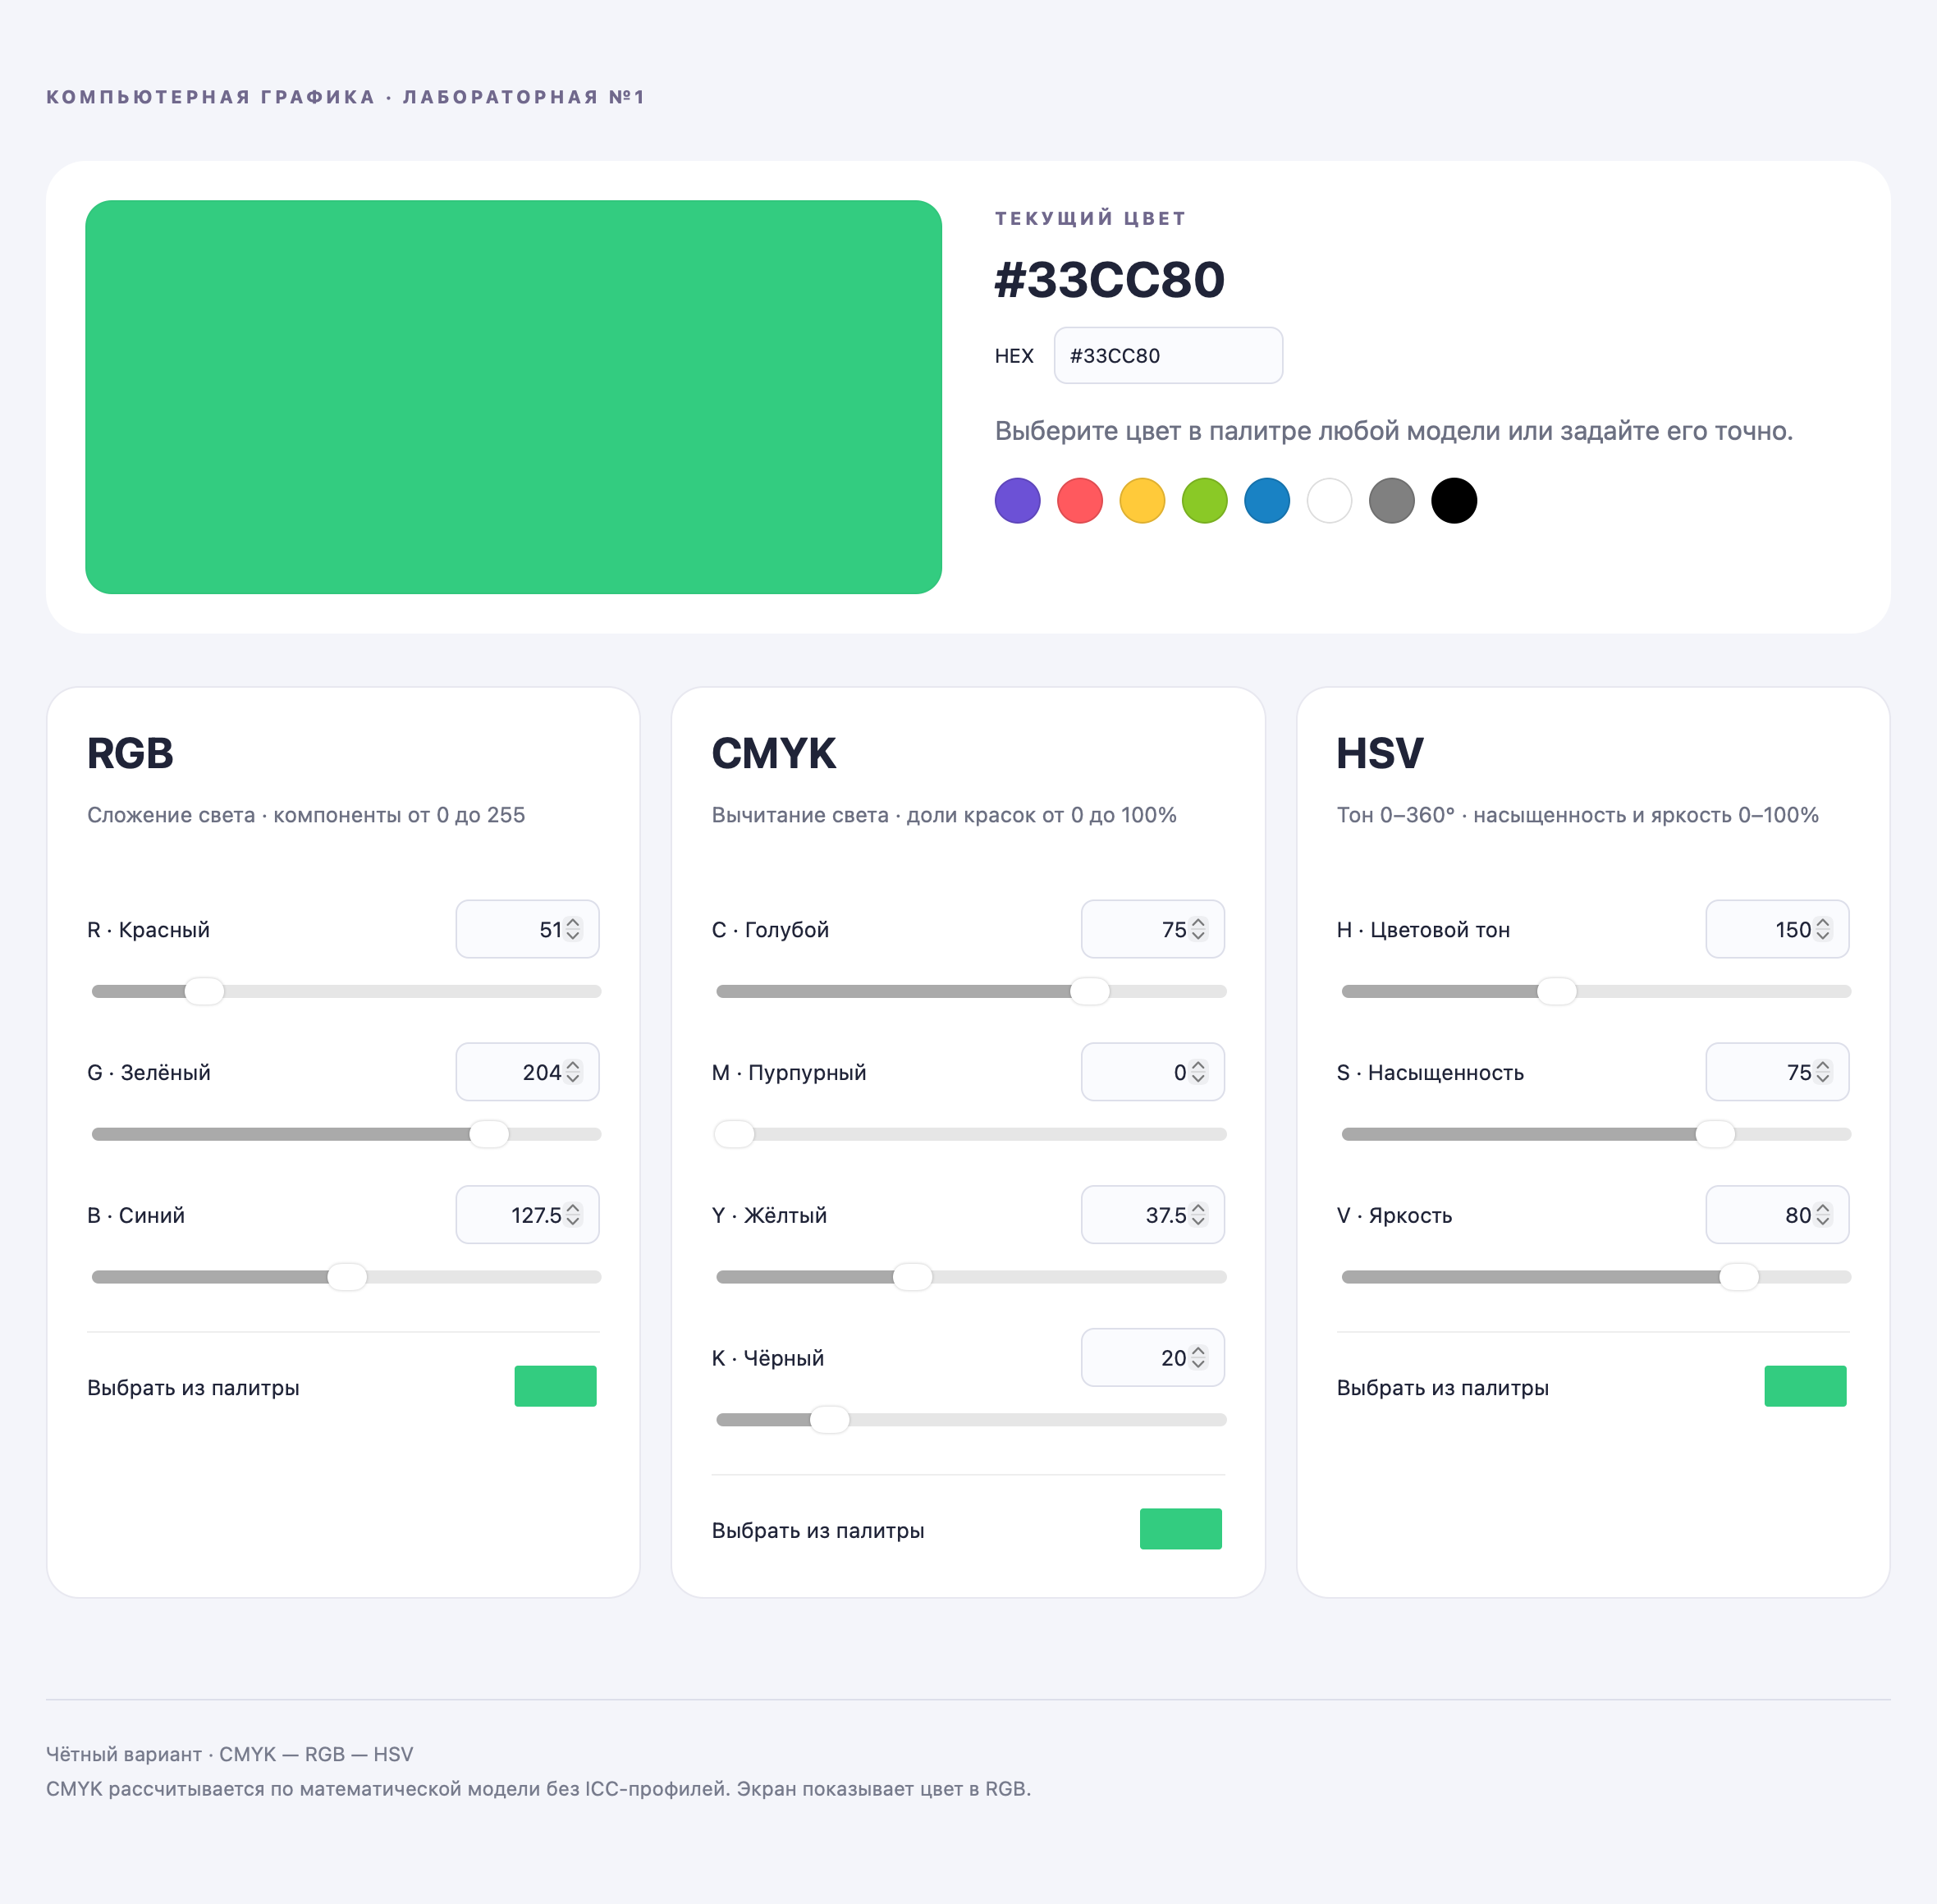
\includegraphics[width=0.66\textwidth]{screenshots/04-hsv.png}\\
{\small Рисунок 4 — HSV $(150,75,80)$; RGB $(51,204,127.5)$.}
\end{center}
\section{Вывод}
Разработано приложение для выбора и изменения цвета в моделях RGB, CMYK и HSV. Реализованы числовой ввод, ползунки и выбор из палитры, а также автоматический пересчёт представлений. Проверки подтверждают корректность математических преобразований на контрольных и случайных значениях. При реализации учтены особенности чёрного и ахроматических цветов, циклический диапазон тона и неоднозначность представления CMYK.

\end{document}
